\documentclass[11pt,a4paper]{article}

\usepackage[a4paper,margin=2.3cm]{geometry}
\usepackage[T1]{fontenc}
\usepackage{lmodern}
\usepackage{microtype}
\usepackage{amsmath,amssymb}
\usepackage{graphicx}
\usepackage{booktabs}
\usepackage{float}
\usepackage[font=small,labelfont=bf]{caption}
\usepackage{enumitem}
\usepackage{titlesec}
\usepackage{xcolor}
\usepackage{listings}
\usepackage[hidelinks]{hyperref}

\graphicspath{{../figures/}{./}}
\setlength{\parindent}{0pt}
\setlength{\parskip}{5pt}
\linespread{1.08}
\setlist{itemsep=1pt,topsep=2pt}

\titleformat{\section}{\Large\bfseries}{\thesection.}{0.5em}{}
\titleformat{\subsection}{\large\bfseries}{\thesubsection}{0.5em}{}
\renewcommand{\thesubsection}{\thesection(\alph{subsection})}
\titlespacing*{\section}{0pt}{16pt}{6pt}
\titlespacing*{\subsection}{0pt}{10pt}{4pt}

\definecolor{codebg}{RGB}{247,247,247}
\definecolor{codekw}{RGB}{0,90,160}
\definecolor{codecm}{RGB}{110,110,110}
\definecolor{codestr}{RGB}{163,21,21}
\lstset{
  language=Python, basicstyle=\ttfamily\footnotesize, keywordstyle=\color{codekw}\bfseries,
  commentstyle=\color{codecm}\itshape, stringstyle=\color{codestr}, backgroundcolor=\color{codebg},
  frame=single, rulecolor=\color{black!15}, framesep=4pt, xleftmargin=4pt, xrightmargin=4pt,
  breaklines=true, columns=fullflexible, keepspaces=true, showstringspaces=false,
  aboveskip=6pt, belowskip=6pt
}

% no headers, footers or page numbers on any page
\pagestyle{empty}

\begin{document}

% ====================================================================
%                              COVER PAGE
% ====================================================================
\begin{titlepage}
  \centering
  \vspace*{0.5cm}
  
\includegraphics[width=4.2cm]{uom_logo.png}\par
  \vspace{0.8cm}
  {\LARGE\bfseries UNIVERSITY OF MORATUWA\par}
  \vspace{0.25cm}
  {\large Faculty of Engineering\par}
  \vspace{0.1cm}
  {\large Department of Electronic and Telecommunication Engineering\par}

  \vspace{1.6cm}
  \rule{\textwidth}{1.2pt}\par
  \vspace{0.4cm}
  {\Large\bfseries EN4554\par}
  \vspace{0.3cm}
  {\huge\bfseries Assignment 2\par}
  \vspace{0.3cm}
  {\large Convolutional Neural Networks on CIFAR-10\par}
  \vspace{0.3cm}
  \rule{\textwidth}{1.2pt}\par

  \vspace{2.2cm}
  {\large
  \begin{tabular}{@{}l@{\hspace{1.2em}}l@{}}
    \textbf{Name}       & : \ Eashan S.G.S \\[6pt]
    \textbf{Index No.}  & : \ 220148G
  \end{tabular}\par}

  \vfill
\end{titlepage}

% ====================================================================
\section*{Overview}

\textbf{GitHub repository:} \url{https://github.com/sahas-eashan/EN4554-Assignment-2-CNNs}\\
The repository holds the full Jupyter notebook (\texttt{220148G\_a02.ipynb}) with every cell output. This report shows the important parts of the code, the results and their interpretation.

\textbf{Setup.}
\begin{itemize}
  \item \textbf{Framework:} PyTorch, run on an NVIDIA RTX 3090.
  \item \textbf{Data split:} the CIFAR-10 training set is split into \textbf{45k train / 5k validation} with a fixed seed.
  \item \textbf{Normalization:} per channel, using the statistics of the 45k training split only: mean $(0.491, 0.482, 0.446)$, standard deviation $(0.247, 0.244, 0.262)$.
  \item \textbf{Data pipeline:} the whole dataset is kept on the GPU, and mini-batching and all augmentations run there.
  \item \textbf{Test set:} used \textbf{once}, in Task~4.
  \item \textbf{Reproducibility:} all random seeds are fixed.
\end{itemize}

\textbf{Use of AI tools.} Claude (Anthropic) was used as a coding assistant to write and debug the code and to help run the experiments on the lab GPU server. I have reviewed and understood all of the code and the results.

\begin{figure}[H]
  \centering
  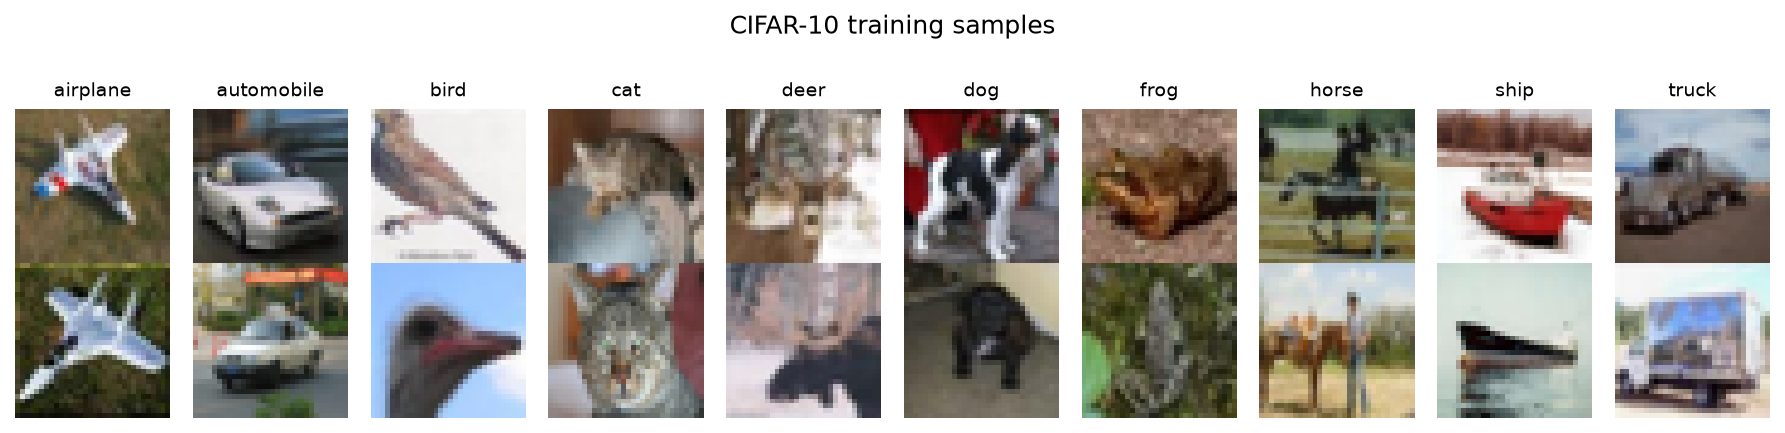
\includegraphics[width=\textwidth]{samples.png}
  \caption{Two training images from each CIFAR-10 class.}
\end{figure}

% ====================================================================
\section{Backpropagation}

\subsection{Layers with explicit forward/backward passes}

Each layer caches what its backward pass needs. For an upstream gradient $\delta=\partial\ell/\partial\,\text{out}$:
\[
\begin{aligned}
&\textbf{Linear } y=xW+b: && \tfrac{\partial\ell}{\partial W}=x^\top\delta,\quad \tfrac{\partial\ell}{\partial b}=\textstyle\sum_n\delta_n,\quad \tfrac{\partial\ell}{\partial x}=\delta W^\top\\
&\textbf{ReLU}: && \tfrac{\partial\ell}{\partial x}=\delta\odot\mathbf{1}[x>0]\\
&\textbf{Sigmoid } s=\sigma(x): && \tfrac{\partial\ell}{\partial x}=\delta\odot s(1-s)\\
&\textbf{Softmax CE } \ell=-\tfrac1N\textstyle\sum_n\log p_{n,y_n}: && \tfrac{\partial\ell}{\partial z}=\tfrac1N\big(p-\mathrm{onehot}(y)\big)
\end{aligned}
\]
No autograd is used: none of the tensors require gradients.

\begin{lstlisting}
class Linear:
    def __init__(self, n_in, n_out, init="he", dtype=torch.float32, device=DEVICE):
        # He init for ReLU, Xavier init for sigmoid
        std = math.sqrt(2.0 / n_in) if init == "he" else math.sqrt(2.0 / (n_in + n_out))
        self.W = torch.randn(n_in, n_out, dtype=dtype, device=device) * std
        self.b = torch.zeros(n_out, dtype=dtype, device=device)
    def forward(self, x):
        self.x = x
        return x @ self.W + self.b
    def backward(self, dout):
        self.dW = self.x.T @ dout
        self.db = dout.sum(0)
        return dout @ self.W.T

class ReLU:
    def forward(self, x):
        self.mask = x > 0
        return x * self.mask
    def backward(self, dout):
        return dout * self.mask

class SoftmaxCrossEntropy:
    def forward(self, z, y):
        z = z - z.max(dim=1, keepdim=True).values             # numerical stability
        logp = z - torch.logsumexp(z, dim=1, keepdim=True)
        self.p, self.y = logp.exp(), y
        return -logp[torch.arange(len(y)), y].mean()
    def backward(self):
        g = self.p.clone()
        g[torch.arange(len(self.y)), self.y] -= 1
        return g / len(self.y)
\end{lstlisting}
The \texttt{MLP} class stacks \texttt{Linear} and activation layers. Its \texttt{backward()} walks the layers in reverse, passing each layer's input gradient to the layer below.

% --------------------------------------------------------------------
\subsection{Gradient check}

A small MLP (20--16--12--10, ReLU) was checked in float64 on a random batch of 8 samples. The manual gradients were compared against:
\begin{enumerate}
  \item \textbf{autograd}, using the same weights in an equivalent PyTorch network;
  \item \textbf{centred finite differences}, $\frac{\ell(\theta_i+\varepsilon)-\ell(\theta_i-\varepsilon)}{2\varepsilon}$ with $\varepsilon=10^{-6}$, for \emph{every} parameter.
\end{enumerate}
The relative error is $\|g_1-g_2\|_2/(\|g_1\|_2+\|g_2\|_2)$.

\begin{lstlisting}
def finite_diff(net, x, y, eps=1e-6):
    out = []
    for p in net.params():
        flat, g = p.view(-1), torch.zeros(p.numel(), dtype=p.dtype)
        for i in range(flat.numel()):
            old = flat[i].item()
            flat[i] = old + eps; lp = net.loss(x, y).item()
            flat[i] = old - eps; lm = net.loss(x, y).item()
            flat[i] = old
            g[i] = (lp - lm) / (2 * eps)
        out.append(g.view_as(p))
    return out
\end{lstlisting}

\begin{table}[H]
\centering
\caption{Gradient check (loss: manual $3.757791109124$, autograd $3.757791109124$).}
\begin{tabular}{lccccc}
\toprule
parameter & shape & rel.\ err vs autograd & \texttt{allclose} & rel.\ err vs finite diff. & \texttt{allclose}\\
\midrule
$W_1$ & $20\times16$ & $4.57\times10^{-17}$ & True & $6.13\times10^{-10}$ & True\\
$b_1$ & $16$         & $5.98\times10^{-17}$ & True & $5.00\times10^{-10}$ & True\\
$W_2$ & $16\times12$ & $1.94\times10^{-17}$ & True & $3.99\times10^{-10}$ & True\\
$b_2$ & $12$         & $2.54\times10^{-17}$ & True & $3.51\times10^{-10}$ & True\\
$W_3$ & $12\times10$ & $1.31\times10^{-17}$ & True & $4.40\times10^{-10}$ & True\\
$b_3$ & $10$         & $2.31\times10^{-17}$ & True & $1.00\times10^{-9}$  & True\\
\bottomrule
\end{tabular}
\end{table}

\textbf{Interpretation.}
\begin{itemize}
  \item \textbf{Against autograd:} the manual gradients agree to machine precision (about $10^{-17}$), the two losses are identical to 12 digits, and \texttt{torch.allclose} passes for every parameter.
  \item \textbf{Against finite differences:} the errors of $10^{-10}$--$10^{-9}$ are exactly the expected $O(\varepsilon^2)$ truncation error plus round-off.
  \item The finite-difference check uses no framework, so it validates the derivations themselves, not just consistency with PyTorch.
\end{itemize}

% --------------------------------------------------------------------
\subsection{Training the MLP with SGD}

The from-scratch MLP is 3072--512--256--10 with ReLU and He initialization. It is trained on flattened images with plain mini-batch SGD (batch 128, learning rate 0.02, 20 epochs), using a hand-written update:
\begin{lstlisting}
for xb, yb in batches(Xf_tr, Ytr, bs):
    loss = net.loss(xb, yb)
    net.backward()
    for p, g in zip(net.params(), net.grads()):
        p -= lr * g                        # plain SGD step (in place)
\end{lstlisting}

\begin{figure}[H]
  \centering
  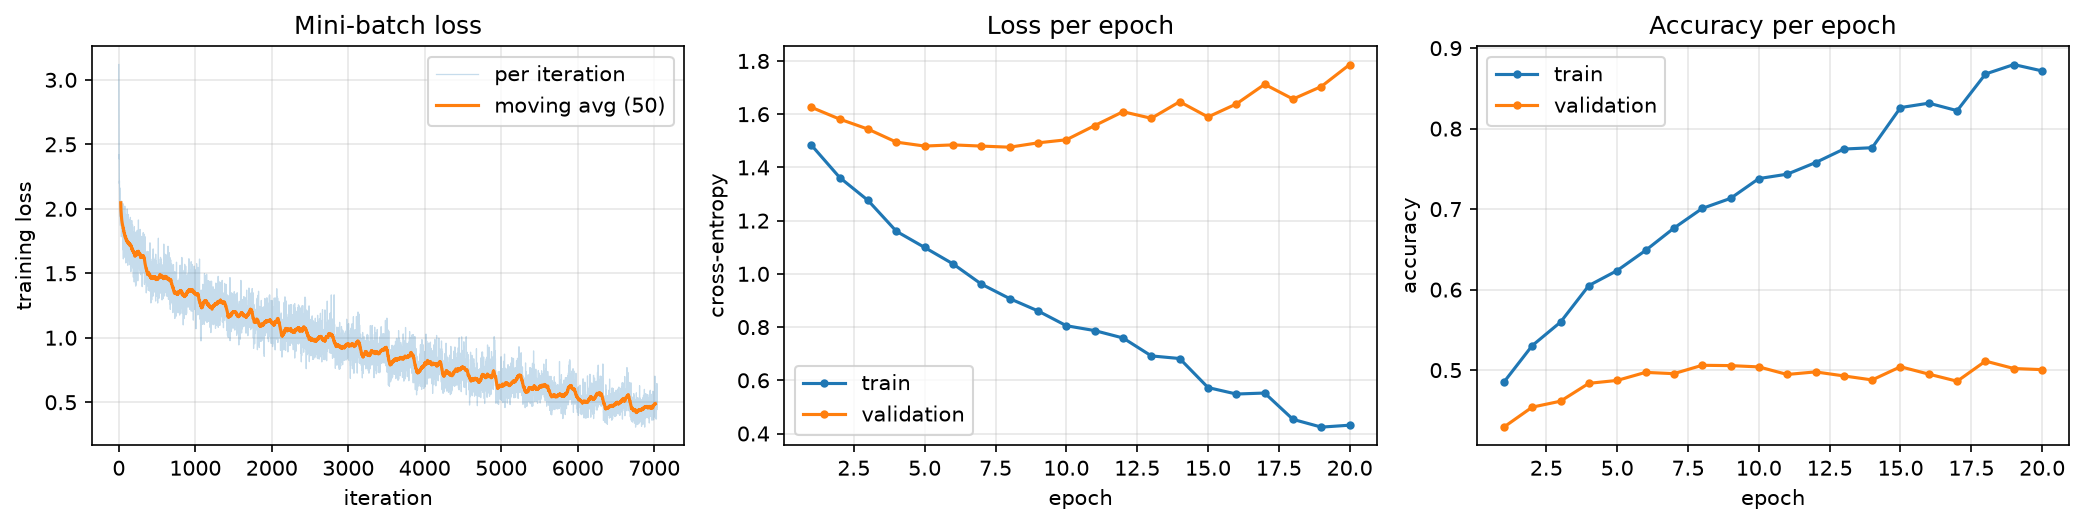
\includegraphics[width=\textwidth]{t1c_mlp.png}
  \caption{From-scratch MLP: mini-batch loss, per-epoch loss and per-epoch accuracy.}
\end{figure}

\textbf{Result:} best validation accuracy \textbf{51.1\,\%} (epoch 18); final validation accuracy \textbf{50.1\,\%}.

\textbf{Interpretation.}
\begin{itemize}
  \item \textbf{Loss curve:} the mini-batch loss drops quickly from 2.3 to about 1.5 in the first epoch, then falls steadily to about 0.5. The noise around the moving average comes from SGD sampling.
  \item \textbf{Accuracy:} about 50\,\% is typical for a fully connected network on raw pixels. Flattening discards spatial structure, and without weight sharing every pattern must be learned separately at every position.
  \item \textbf{Overfitting:}
  \begin{itemize}
    \item The validation loss reaches its minimum (about 1.47) around epochs 5--8 and then rises to 1.78.
    \item Over the same period the training accuracy climbs to 87\,\% while validation accuracy stays flat near 50\,\%.
    \item The 1.7M-parameter MLP is memorizing the training set, so early stopping or regularization would be needed.
  \end{itemize}
\end{itemize}

% --------------------------------------------------------------------
\subsection{Gradient norms at initialization: sigmoid vs ReLU}

The test network is a 10-layer MLP: 3072 inputs, 9 hidden layers of width 256, and 10 outputs.
\begin{itemize}
  \item The sigmoid version uses Xavier initialization and the ReLU version uses He initialization, i.e.\ each activation gets its standard initialization.
  \item One forward/backward pass on 512 training images gives $\|\partial\ell/\partial W_l\|_F$ for every layer.
\end{itemize}

\begin{figure}[H]
  \centering
  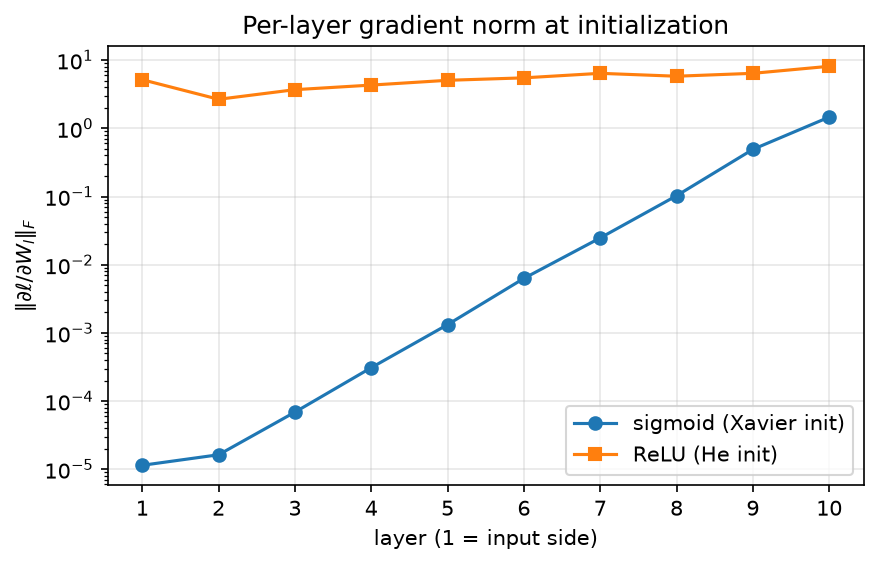
\includegraphics[width=0.62\textwidth]{t1d_gradnorms.png}
  \caption{Per-layer weight-gradient norm at initialization (log scale).}
\end{figure}

\begin{table}[H]
\centering\small
\caption{$\|\partial\ell/\partial W_l\|_F$ per layer (layer 1 = input side).}
\setlength{\tabcolsep}{3.5pt}
\begin{tabular}{lcccccccccc}
\toprule
layer & 1 & 2 & 3 & 4 & 5 & 6 & 7 & 8 & 9 & 10\\
\midrule
sigmoid & 1.2e-5 & 1.6e-5 & 6.9e-5 & 3.1e-4 & 1.3e-3 & 6.3e-3 & 2.5e-2 & 0.10 & 0.49 & 1.46\\
ReLU    & 5.16 & 2.66 & 3.69 & 4.30 & 5.06 & 5.49 & 6.40 & 5.80 & 6.40 & 8.11\\
\bottomrule
\end{tabular}
\end{table}

\textbf{Interpretation.}
\begin{itemize}
  \item \textbf{Sigmoid:} the gradient norm falls by about \textbf{five orders of magnitude} from the output layer to the input layer (layer-1/layer-10 ratio $7.8\times10^{-6}$). This is the \textbf{vanishing-gradient} problem.
  \begin{itemize}
    \item Each backward step multiplies the gradient by $\sigma'(z)\le0.25$, and by $W^\top$, whose gain under Xavier initialization is about 1.
    \item The gradient therefore shrinks by roughly 4$\times$ per layer, which is the straight line on the log plot, and the early layers barely learn.
  \end{itemize}
  \item \textbf{ReLU:} the norms stay within 2.7--8.1 across all layers (ratio 0.64).
  \begin{itemize}
    \item $\mathrm{ReLU}'\in\{0,1\}$, so about half the units pass the gradient through unchanged.
    \item He initialization ($\mathrm{Var}(W)=2/n_\text{in}$) compensates exactly for that factor $\tfrac12$, so the gradient variance is preserved with depth.
  \end{itemize}
\end{itemize}

% ====================================================================
\section{Optimizers}

\subsection{SGD with momentum and Adam as \texttt{torch.optim.Optimizer} subclasses}

For a gradient $g_t$ (with L2 weight decay, $g_t\leftarrow g_t+\lambda\theta$):
\begin{itemize}
  \item \textbf{SGD with momentum:} $b_t=\mu b_{t-1}+g_t$, $\;\theta\leftarrow\theta-\eta b_t$, with $b_1=g_1$.
  \item \textbf{Adam:} $m_t=\beta_1m_{t-1}+(1-\beta_1)g_t$, $\;v_t=\beta_2v_{t-1}+(1-\beta_2)g_t^2$. The bias-corrected moments are $\hat m_t=m_t/(1-\beta_1^t)$ and $\hat v_t=v_t/(1-\beta_2^t)$, and the update is $\theta\leftarrow\theta-\eta\,\hat m_t/(\sqrt{\hat v_t}+\epsilon)$.
\end{itemize}

\begin{lstlisting}
class MySGD(torch.optim.Optimizer):
    def __init__(self, params, lr=1e-2, momentum=0.0, weight_decay=0.0):
        super().__init__(params, dict(lr=lr, momentum=momentum, weight_decay=weight_decay))
    @torch.no_grad()
    def step(self, closure=None):
        for group in self.param_groups:
            lr, mu, wd = group["lr"], group["momentum"], group["weight_decay"]
            for p in group["params"]:
                if p.grad is None:
                    continue
                g = p.grad if wd == 0 else p.grad.add(p, alpha=wd)
                if mu != 0:
                    state = self.state[p]
                    if "buf" not in state:
                        state["buf"] = g.clone()
                    else:
                        state["buf"].mul_(mu).add_(g)
                    g = state["buf"]
                p.add_(g, alpha=-lr)

class MyAdam(torch.optim.Optimizer):
    def __init__(self, params, lr=1e-3, betas=(0.9, 0.999), eps=1e-8, weight_decay=0.0):
        super().__init__(params, dict(lr=lr, betas=betas, eps=eps, weight_decay=weight_decay))
    @torch.no_grad()
    def step(self, closure=None):
        for group in self.param_groups:
            lr, (b1, b2) = group["lr"], group["betas"]
            eps, wd = group["eps"], group["weight_decay"]
            for p in group["params"]:
                if p.grad is None:
                    continue
                g = p.grad if wd == 0 else p.grad.add(p, alpha=wd)
                state = self.state[p]
                if not state:
                    state["t"] = 0
                    state["m"] = torch.zeros_like(p)
                    state["v"] = torch.zeros_like(p)
                state["t"] += 1
                t, m, v = state["t"], state["m"], state["v"]
                m.mul_(b1).add_(g, alpha=1 - b1)
                v.mul_(b2).addcmul_(g, g, value=1 - b2)
                m_hat, v_hat = m / (1 - b1 ** t), v / (1 - b2 ** t)
                p.addcdiv_(m_hat, v_hat.sqrt().add_(eps), value=-lr)
\end{lstlisting}
(The closure handling is omitted here; it is in the notebook.)

\textbf{Equivalence test.} Two copies of the same float64 network are trained side by side for 200 steps on identical mini-batches, one with my optimizer and one with the \texttt{torch.optim} reference.

\begin{table}[H]
\centering
\caption{Custom vs.\ PyTorch optimizers after 200 steps.}
\begin{tabular}{lcc}
\toprule
configuration & max $|\theta_\text{mine}-\theta_\text{torch}|$ & \texttt{torch.allclose}\\
\midrule
SGD ($\eta=0.1$) & 0 & True\\
SGD momentum ($\eta=0.05$, $\mu=0.9$, wd $10^{-3}$) & 0 & True\\
Adam ($\eta=10^{-2}$) & $4.4\times10^{-16}$ & True\\
Adam ($\eta=10^{-3}$, $\beta=(0.8,0.99)$, wd $10^{-3}$) & $8.3\times10^{-17}$ & True\\
\bottomrule
\end{tabular}
\end{table}

\textbf{Interpretation.}
\begin{itemize}
  \item The SGD variants match PyTorch \textbf{bit-for-bit}.
  \item Adam differs only by round-off. PyTorch folds the bias corrections into the step size and the denominator, which is algebraically identical to the textbook form used here.
\end{itemize}

% --------------------------------------------------------------------
\subsection{Trajectories on $f(x,y)=\tfrac12(x^2+50y^2)$}

The Hessian is $\mathrm{diag}(1,50)$, so the condition number is $\kappa=50$. All three methods start from $(-4.5,1)$ and run for 100 steps:
\begin{itemize}
  \item SGD and SGD with momentum ($\mu=0.9$) both use $\eta=0.03$. Gradient descent is stable only for $\eta<2/50$.
  \item Adam uses $\eta=0.3$.
\end{itemize}
The gradient is exact, so ``SGD'' here is plain gradient descent.

\begin{figure}[H]
  \centering
  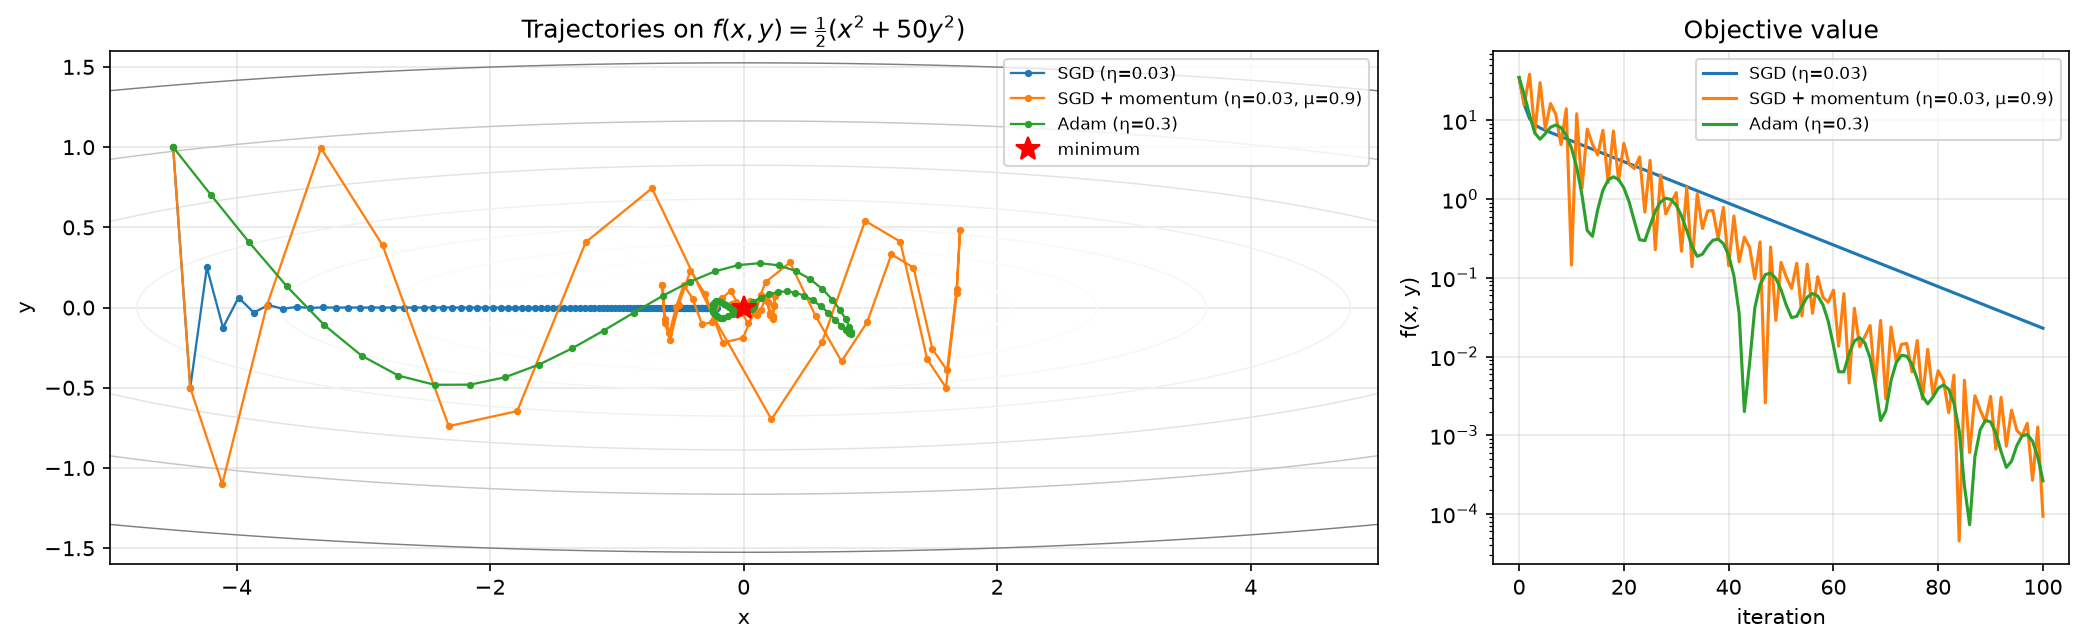
\includegraphics[width=\textwidth]{t2b_trajectories.png}
  \caption{Optimizer trajectories over the contours of $f$ (left) and the objective value per iteration (right).}
\end{figure}

\begin{table}[H]
\centering
\caption{Position and objective after 100 steps.}
\begin{tabular}{lcc}
\toprule
optimizer & final $(x,y)$ & $f(x,y)$\\
\midrule
SGD ($\eta=0.03$) & $(-0.214,\ 0.000)$ & $2.29\times10^{-2}$\\
SGD + momentum ($\eta=0.03$, $\mu=0.9$) & $(0.011,\ -0.001)$ & $9.34\times10^{-5}$\\
Adam ($\eta=0.3$) & $(-0.020,\ -0.002)$ & $2.63\times10^{-4}$\\
\bottomrule
\end{tabular}
\end{table}

\textbf{Interpretation.}
\begin{itemize}
  \item \textbf{SGD:}
  \begin{itemize}
    \item Along the steep $y$ direction each step multiplies the error by $1-50\eta=-0.5$. The first steps zig-zag across the valley, and $y$ then dies out quickly.
    \item Along the flat $x$ direction the factor is only $0.97$, so the iterate creeps forward and is still at $x=-0.21$ after 100 steps.
    \item A learning rate that is safe for the steep direction is tiny for the flat one. This is the ill-conditioning problem.
  \end{itemize}
  \item \textbf{SGD + momentum:}
  \begin{itemize}
    \item The velocity accumulates the consistent $x$-gradient, giving roughly $1/(1-\mu)=10\times$ faster progress along the valley. The final $f$ is 250$\times$ lower than SGD's.
    \item With $\mu=0.9$ the system is strongly under-damped. The path swings far past the minimum (out to $x\approx1.7$), and $f$ oscillates instead of decreasing monotonically.
  \end{itemize}
  \item \textbf{Adam:}
  \begin{itemize}
    \item Each coordinate is normalized by its own gradient RMS, so the first steps have size about $\eta$ in \emph{both} directions, a diagonal move along $-\mathrm{sign}(\nabla f)$. The steep $y$ direction no longer dictates the step.
    \item The path is smooth. It overshoots to $x\approx0.85$ and then spirals in.
  \end{itemize}
  \item Momentum and adaptive scaling are two different remedies for ill-conditioning. Both beat gradient descent by about two orders of magnitude.
\end{itemize}

% --------------------------------------------------------------------
\subsection{Optimizer comparison on a small CNN}

\textbf{Model:} conv32--conv32--pool--conv64--conv64--pool--conv128--pool--FC256--FC10 (666{,}538 parameters). It has \textbf{no batch norm}, so normalization does not mask the optimizer's behaviour.

\textbf{Training:} each optimizer from 2(a) is trained at $\eta\in\{10^{-3},10^{-2},10^{-1}\}$ for 10 epochs on the 45k training split, with batch size 128, a constant learning rate and no augmentation.

\begin{table}[H]
\centering
\caption{Validation accuracy after 10 epochs (best per optimizer in bold).}
\begin{tabular}{lccc}
\toprule
optimizer & $\eta=10^{-3}$ & $\eta=10^{-2}$ & $\eta=10^{-1}$\\
\midrule
SGD & 13.6\,\% & 43.8\,\% & \textbf{68.0\,\%}\\
SGD + momentum & 47.6\,\% & \textbf{74.9\,\%} & 55.2\,\%\\
Adam & \textbf{75.1\,\%} & 52.4\,\% & 10.0\,\%\\
\bottomrule
\end{tabular}
\end{table}

\begin{figure}[H]
  \centering
  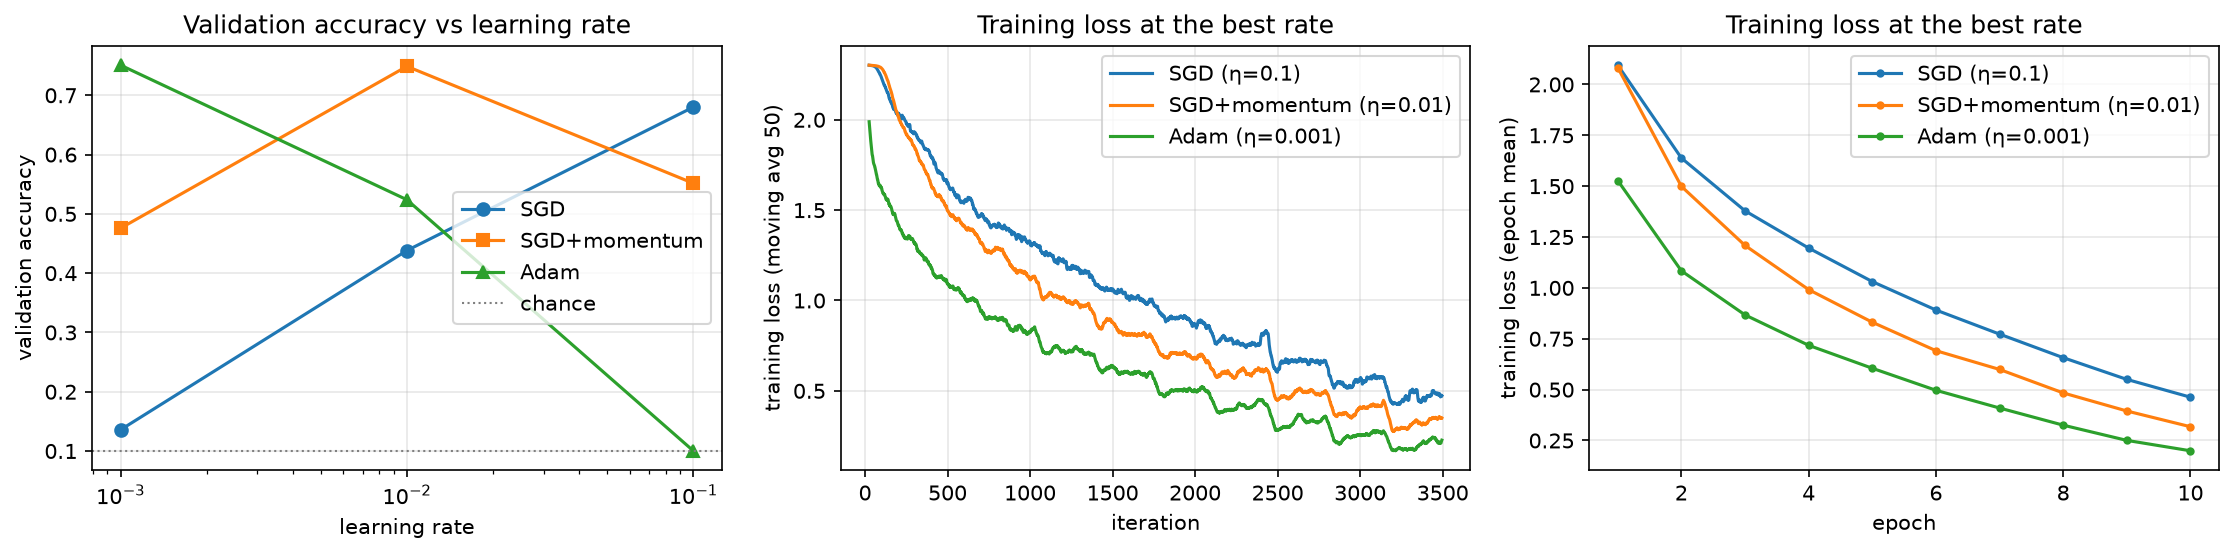
\includegraphics[width=\textwidth]{t2c_optimizers.png}
  \caption{Validation accuracy versus learning rate (left), and training loss at each optimizer's best rate (middle and right).}
\end{figure}

\textbf{Interpretation.}
\begin{itemize}
  \item \textbf{Each optimizer has its own sweet spot,} one decade lower for each step from SGD to momentum to Adam:
  \begin{itemize}
    \item Momentum's effective step is about $\eta/(1-\mu)=10\eta$, so it wants a 10$\times$ smaller rate than SGD.
    \item Adam normalizes every update to about $\eta$ per parameter, so it needs the smallest rate.
  \end{itemize}
  \item \textbf{High sensitivity:} one decade away from the best rate costs 25--65 points.
  \begin{itemize}
    \item SGD at $10^{-3}$ barely leaves chance level (13.6\,\%).
    \item Adam at $10^{-1}$ never learns: its loss stays at $\ln10\approx2.30$ (chance), as the huge per-parameter steps immediately drive the ReLUs into a dead or saturated state.
    \item SGD's best rate is at the edge of the grid, so it would probably improve further at a higher rate.
  \end{itemize}
  \item \textbf{Best results:} at their best rates, Adam and momentum both reach about \textbf{75\,\%}, ahead of plain SGD (68\,\%).
  \item \textbf{Training speed:} Adam reduces the training loss fastest throughout, followed by momentum and then plain SGD. Faster convergence only holds when the learning rate is tuned per optimizer.
\end{itemize}

% ====================================================================
\section{Regularization and Residual Connections}

\subsection{Regularization on 5k training images}

\textbf{Setup:}
\begin{itemize}
  \item \textbf{Data:} a class-balanced subset of 5{,}000 training images (500 per class). Evaluation uses the 5k validation split.
  \item \textbf{Model:} the SmallCNN from 2(c) \textbf{with batch norm}.
  \item \textbf{Training:} SGD with momentum 0.9, learning rate 0.05 with cosine decay, batch size 128, 60 epochs.
  \item \textbf{Settings compared:}
  \begin{itemize}
    \item weight decay $10^{-3}$;
    \item dropout $p=0.5$ on the FC layers;
    \item random flip + 4-pixel-padded crop;
    \item cutout (one 16$\times$16 hole);
    \item mixup ($\alpha=0.4$);
    \item all of these combined.
  \end{itemize}
  \item \textbf{Train accuracy} is measured on the clean training images in eval mode, so it is comparable across settings.
\end{itemize}

Cutout and mixup are my own implementations, applied per batch on the GPU:
\begin{lstlisting}
def cutout(x, size=16):
    B, C, H, W = x.shape
    cy = torch.randint(0, H, (B, 1, 1), device=x.device)
    cx = torch.randint(0, W, (B, 1, 1), device=x.device)
    yy = torch.arange(H, device=x.device)[None, :, None]
    xx = torch.arange(W, device=x.device)[None, None, :]
    hole = ((yy >= cy - size // 2) & (yy < cy + size // 2) &
            (xx >= cx - size // 2) & (xx < cx + size // 2))
    return x * (~hole)[:, None].to(x.dtype)

def mixup(x, y, alpha):
    lam = float(np.random.beta(alpha, alpha))
    j = torch.randperm(len(x), device=x.device)
    return lam * x + (1 - lam) * x[j], y, y[j], lam
# loss = lam * CE(out, y) + (1 - lam) * CE(out, y[j])
\end{lstlisting}

\begin{table}[H]
\centering
\caption{Regularization results on 5k training images (60 epochs).}
\begin{tabular}{lcccc}
\toprule
setting & train acc & val acc & gap & best val acc\\
\midrule
baseline & 100.0\,\% & 66.5\,\% & 33.5 & 66.5\,\%\\
weight decay & 100.0\,\% & 66.9\,\% & 33.1 & 67.2\,\%\\
dropout & 93.9\,\% & 67.3\,\% & 26.6 & 67.7\,\%\\
flip+crop & 93.3\,\% & \textbf{74.7\,\%} & 18.6 & \textbf{75.0\,\%}\\
cutout & 99.9\,\% & 70.1\,\% & 29.8 & 70.3\,\%\\
mixup & 99.9\,\% & 67.4\,\% & 32.5 & 67.7\,\%\\
all combined & 67.3\,\% & 62.8\,\% & \textbf{4.5} & 63.4\,\%\\
\bottomrule
\end{tabular}
\end{table}

\begin{figure}[H]
  \centering
  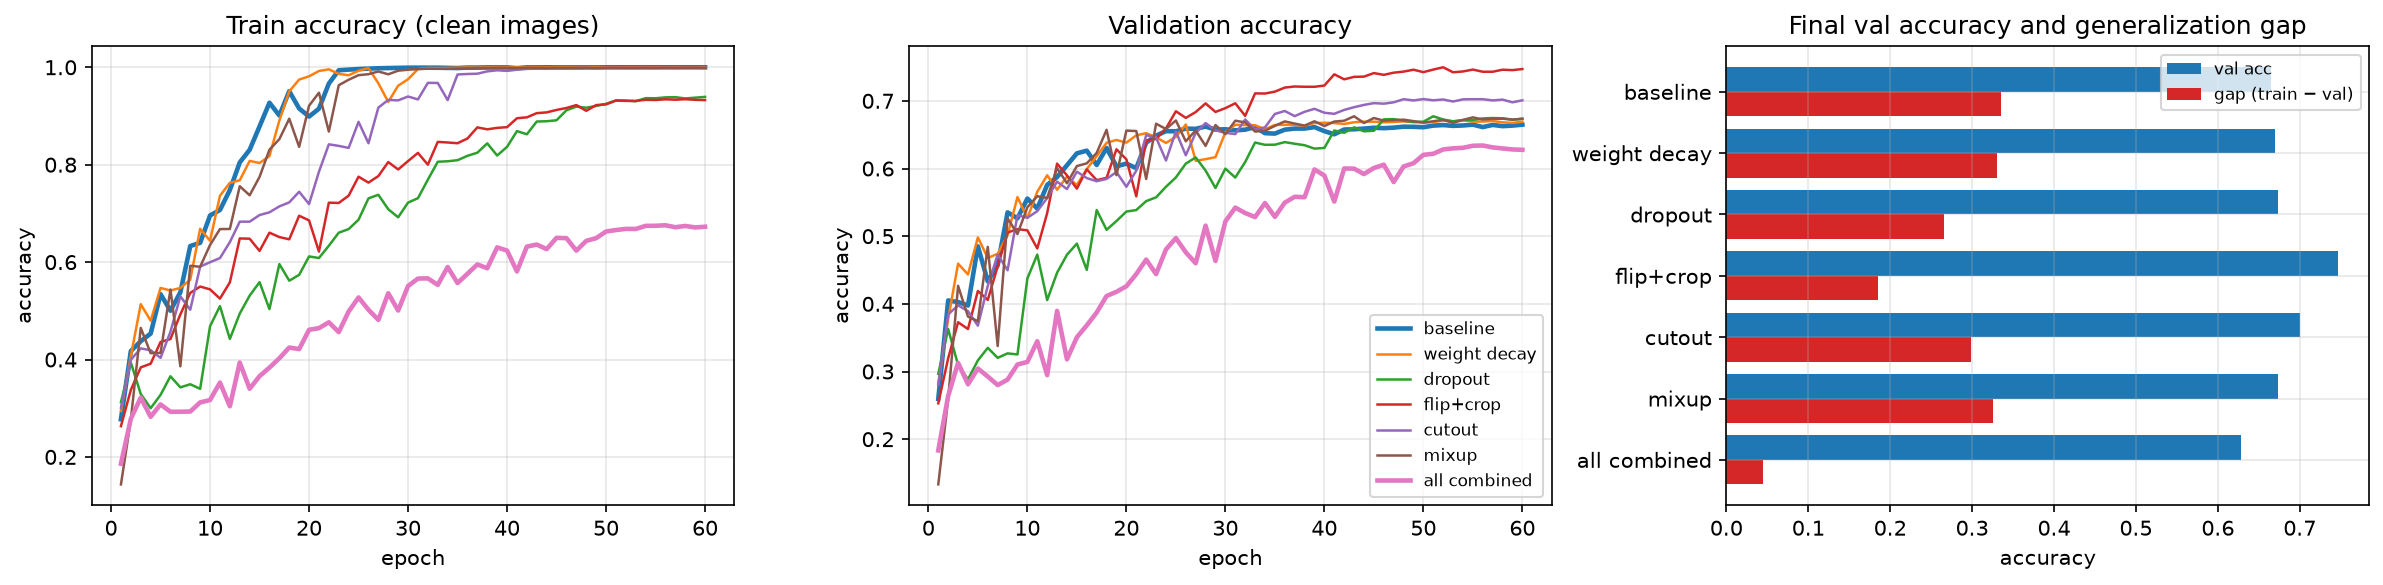
\includegraphics[width=\textwidth]{t3a_regularization.png}
  \caption{Training accuracy (clean images) and validation accuracy per epoch, and the final validation accuracy and generalization gap.}
\end{figure}

\textbf{Interpretation.}
\begin{itemize}
  \item \textbf{Baseline:} the BN-CNN reaches 100\,\% training accuracy by about epoch 25, while validation accuracy plateaus at 66.5\,\%. A 33-point gap means the network has memorized the 5k images.
  \item \textbf{Weight decay:} almost no effect (+0.4 points). With batch norm, the scale of the conv weights does not change the function, so L2 mainly alters the effective learning rate rather than limiting capacity.
  \item \textbf{Dropout:} slows memorization (training accuracy 94\,\%) and shrinks the gap to 27 points, but adds only 0.8 points of validation accuracy.
  \item \textbf{Flip+crop:} by far the best single method (\textbf{+8.2 points}, gap 19). Its label-preserving variants match real invariances of natural images, which effectively enlarges the dataset.
  \item \textbf{Cutout:} also helps (+3.6 points).
  \item \textbf{Mixup:} with $\alpha=0.4$ it barely regularizes here (+0.9 points); clean training accuracy is still 99.9\,\%.
  \item \textbf{All combined:} gives the smallest gap (4.5 points) but the \emph{lowest} validation accuracy, 62.8\,\%. The model \textbf{underfits}: training accuracy is only 67\,\% and still rising at epoch 60.
  \begin{itemize}
    \item Regularization trades variance for bias, and stacking everything would need a longer schedule or weaker settings.
    \item A small gap alone does not mean good generalization.
  \end{itemize}
\end{itemize}

% --------------------------------------------------------------------
\subsection{Plain vs.\ residual networks of depth $6n+2$}

\textbf{Architecture} (CIFAR ResNet of He et al.):
\begin{itemize}
  \item a 3$\times$3 conv stem with 16 channels;
  \item three stages of $n$ basic blocks with 16/32/64 channels, where each block is conv--BN--ReLU--conv--BN (+ shortcut) followed by ReLU;
  \item global average pooling and an FC layer;
  \item Kaiming initialization;
  \item depths 8, 20 and 56 ($n=1,3,9$).
\end{itemize}

The \textbf{only difference between the two families is the identity shortcut}. Where the shape changes, it subsamples and zero-pads the channels (option A), so it adds no parameters.

\textbf{Training (identical for all six networks):}
\begin{itemize}
  \item flip+crop augmentation;
  \item SGD with momentum 0.9 and learning rate 0.1, with a 2-epoch linear warm-up then cosine decay;
  \item weight decay $10^{-4}$, batch size 128;
  \item 30 epochs with mixed precision.
\end{itemize}

\begin{lstlisting}
class BasicBlock(nn.Module):
    def __init__(self, cin, cout, stride, residual):
        super().__init__()
        self.conv1, self.bn1 = conv3x3(cin, cout, stride), nn.BatchNorm2d(cout)
        self.conv2, self.bn2 = conv3x3(cout, cout), nn.BatchNorm2d(cout)
        self.residual, self.stride, self.extra = residual, stride, cout - cin
    def shortcut(self, x):   # option A: parameter-free identity / subsample + zero-pad channels
        if self.stride != 1:
            x = x[:, :, ::self.stride, ::self.stride]
        if self.extra:
            x = F.pad(x, (0, 0, 0, 0, self.extra // 2, self.extra - self.extra // 2))
        return x
    def forward(self, x):
        out = F.relu(self.bn1(self.conv1(x)))
        out = self.bn2(self.conv2(out))
        if self.residual:                # the ONLY difference between plain and residual
            out = out + self.shortcut(x)
        return F.relu(out)
\end{lstlisting}

\begin{table}[H]
\centering
\caption{Plain vs.\ residual networks after 30 epochs (identical parameter counts per depth).}
\begin{tabular}{lcccc}
\toprule
network & parameters & final train loss & final train acc & final val acc\\
\midrule
plain-8 & 75{,}290 & 0.381 & 87.0\,\% & 84.8\,\%\\
residual-8 & 75{,}290 & 0.400 & 86.3\,\% & 84.5\,\%\\
plain-20 & 269{,}722 & 0.224 & 92.4\,\% & 87.5\,\%\\
residual-20 & 269{,}722 & 0.168 & 94.2\,\% & 89.0\,\%\\
plain-56 & 853{,}018 & \textbf{0.685} & 76.1\,\% & 75.7\,\%\\
residual-56 & 853{,}018 & \textbf{0.090} & 97.0\,\% & \textbf{89.9\,\%}\\
\bottomrule
\end{tabular}
\end{table}

\begin{figure}[H]
  \centering
  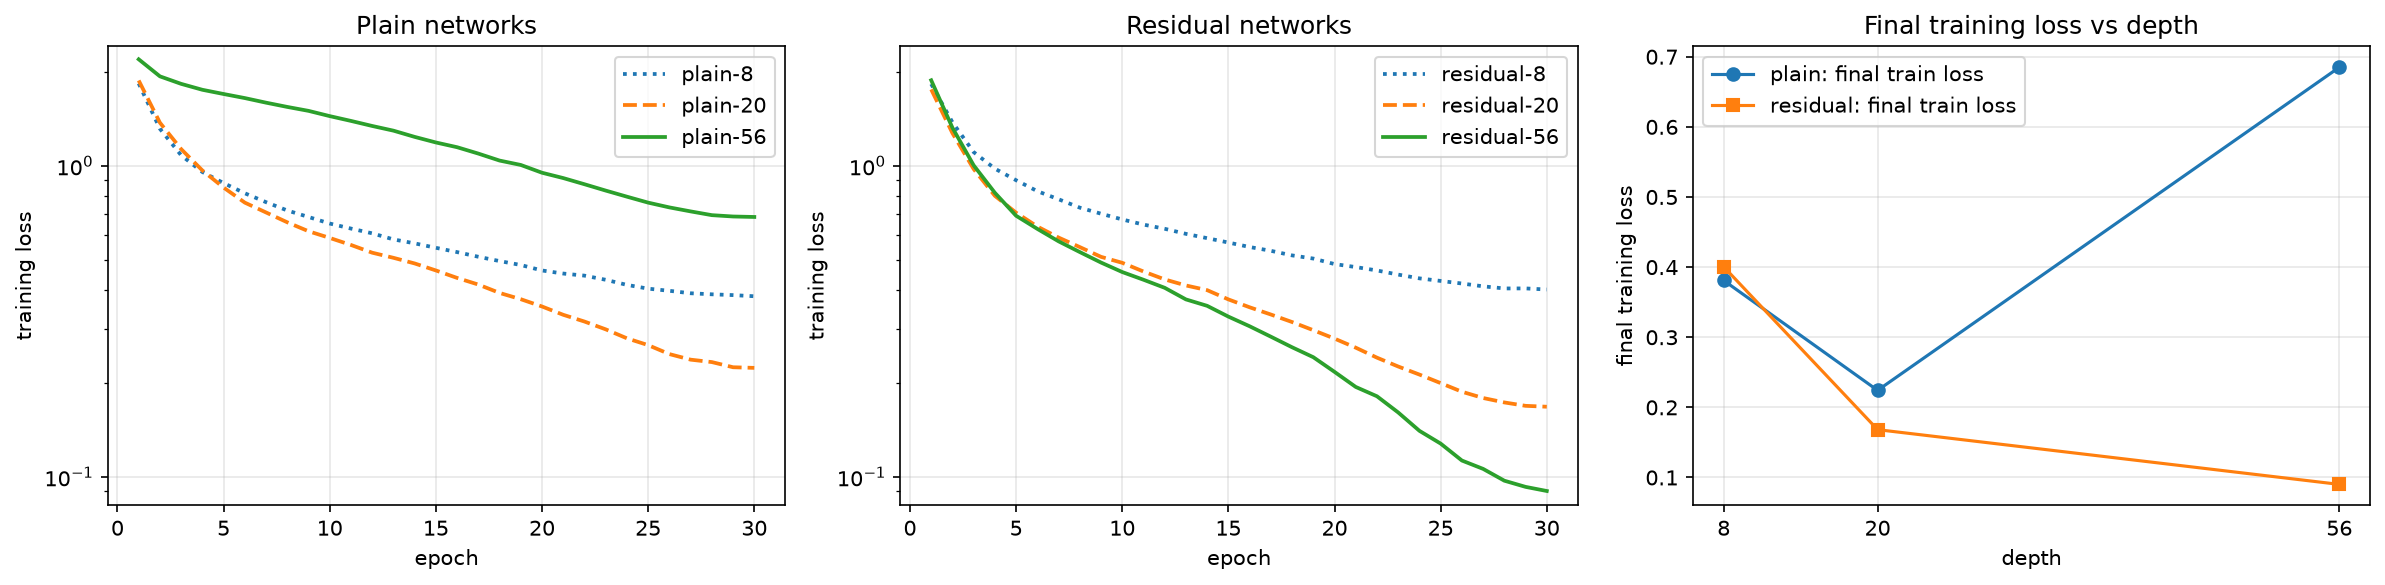
\includegraphics[width=\textwidth]{t3b_plain_vs_residual.png}
  \caption{Training loss per epoch for the plain and residual families, and the final training loss against depth.}
\end{figure}

\textbf{Interpretation.}
\begin{itemize}
  \item \textbf{Plain networks show the degradation problem.}
  \begin{itemize}
    \item Going from 8 to 20 layers helps, but plain-56 is far worse than plain-20: its training loss is 3$\times$ higher, and its curve lies above plain-20's from the first epoch.
    \item The deeper network is worse on the \emph{training} set, so this is an \textbf{optimization failure, not overfitting}. A 56-layer network could in principle copy the 20-layer solution with identity layers, but SGD does not find it.
    \item In a first attempt without warm-up, plain-56 even diverged to NaN in epoch 1, while the residual networks trained normally.
  \end{itemize}
  \item \textbf{Residual networks: deeper is better.} The final training loss falls monotonically with depth (0.400, 0.168, 0.090), and residual-56 is the best network (89.9\,\%).
  \item \textbf{Why the shortcut helps:}
  \begin{itemize}
    \item Each block only learns a residual $F(x)$ on top of $x$, so the identity is the easy default.
    \item The block Jacobian $I+\partial F/\partial x$ gives gradients a direct path to the early layers, instead of a product of 54 conv--BN--ReLU stages.
  \end{itemize}
  \item \textbf{Depth dependence:} at depth 8 the two families are practically identical, and the benefit of the shortcut grows with depth. Parameter counts are identical, so every difference comes from the shortcut alone.
\end{itemize}

% ====================================================================
\section{Best CNN with at most 500k Parameters and 20 Epochs}

\textbf{Design:} a compact ResNet-14.
\begin{itemize}
  \item a 3$\times$3 stem with 32 channels;
  \item three stages of \textbf{2 basic blocks} with \textbf{32/64/96 channels}, stride 2 at the start of stages 2 and 3;
  \item 1$\times$1 projection shortcuts where the shape changes;
  \item global average pooling and an FC layer;
  \item \textbf{481{,}962 parameters} in total.
\end{itemize}

\textbf{Full training recipe:}
\begin{itemize}
  \item 20 epochs, batch size 128;
  \item SGD with Nesterov momentum 0.9 and a one-cycle learning-rate schedule (peak 0.1, 25\,\% warm-up);
  \item weight decay $5\times10^{-4}$;
  \item label smoothing 0.1;
  \item augmentation: flip+crop + cutout;
  \item mixed precision.
\end{itemize}

\textbf{Tuning:} only on the validation split. The test set is evaluated \textbf{once}, for the configuration selected on validation.

\begin{lstlisting}
class Block4(nn.Module):
    def __init__(self, cin, cout, stride, residual=True):
        super().__init__()
        self.conv1, self.bn1 = conv3x3(cin, cout, stride), nn.BatchNorm2d(cout)
        self.conv2, self.bn2 = conv3x3(cout, cout), nn.BatchNorm2d(cout)
        self.residual, self.proj = residual, None
        if residual and (stride != 1 or cin != cout):
            self.proj = nn.Sequential(nn.Conv2d(cin, cout, 1, stride, bias=False),
                                      nn.BatchNorm2d(cout))
    def forward(self, x):
        out = F.relu(self.bn1(self.conv1(x)))
        out = self.bn2(self.conv2(out))
        if self.residual:
            out = out + (x if self.proj is None else self.proj(x))
        return F.relu(out)

opt = torch.optim.SGD(model.parameters(), lr=0.1, momentum=0.9, nesterov=True,
                      weight_decay=5e-4)
h = train(model, opt, 20, Xtr, Ytr, Xva, Yva, bs=128, aug=compose(flip_crop, cutout),
          sched="onecycle", amp=True, label_smoothing=0.1)
\end{lstlisting}

\textbf{Ablation.} Each variant changes exactly one design choice of the full recipe.

\begin{table}[H]
\centering
\caption{Ablation (final validation accuracy after 20 epochs). Full recipe: 89.80\,\%.}
\begin{tabular}{llcc}
\toprule
variant & change & val acc & $\Delta$ vs.\ full\\
\midrule
no augmentation & no flip, crop or cutout & 86.22\,\% & $-3.58$\\
no weight decay & $\lambda=0$ & 88.12\,\% & $-1.68$\\
AdamW & AdamW (peak lr $2\times10^{-3}$, wd 0.05) & 89.40\,\% & $-0.40$\\
no shortcut & plain network (473{,}450 params) & 89.54\,\% & $-0.26$\\
no label smoothing & plain cross-entropy & 90.22\,\% & $+0.42$\\
\textbf{no cutout} & flip+crop only & \textbf{90.78\,\%} & $\mathbf{+0.98}$\\
\bottomrule
\end{tabular}
\end{table}

\begin{figure}[H]
  \centering
  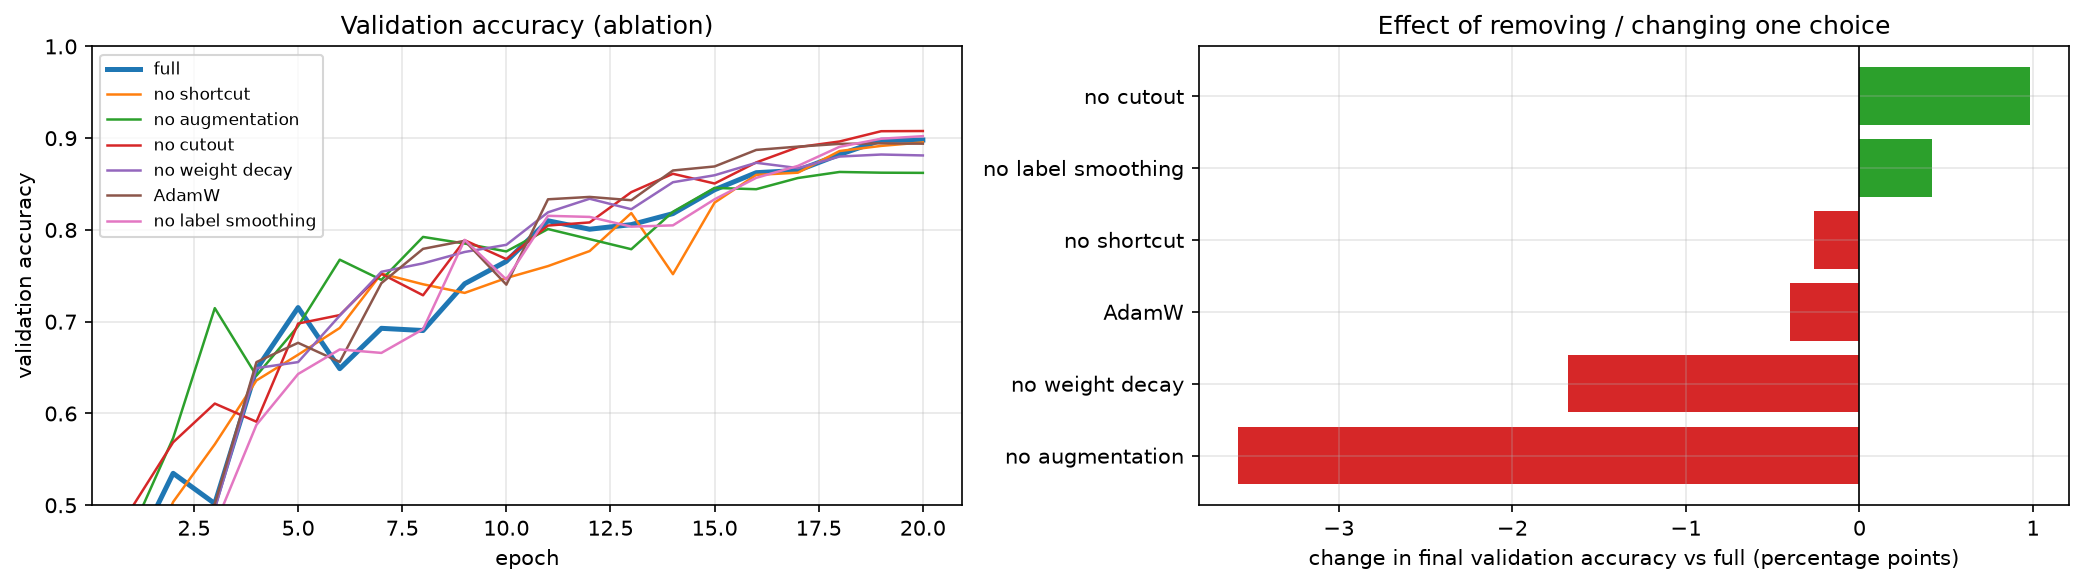
\includegraphics[width=\textwidth]{t4_ablation.png}
  \caption{Validation accuracy per epoch for each variant (left), and the change in final validation accuracy relative to the full recipe (right).}
\end{figure}

\textbf{Final model and test result.} The selected configuration is the full recipe \emph{without cutout}: 481{,}962 parameters, 20 epochs, 90.78\,\% validation accuracy. Its single test-set evaluation gives
\[
\boxed{\text{Test accuracy} = 91.23\,\%}
\]

\begin{figure}[H]
  \centering
  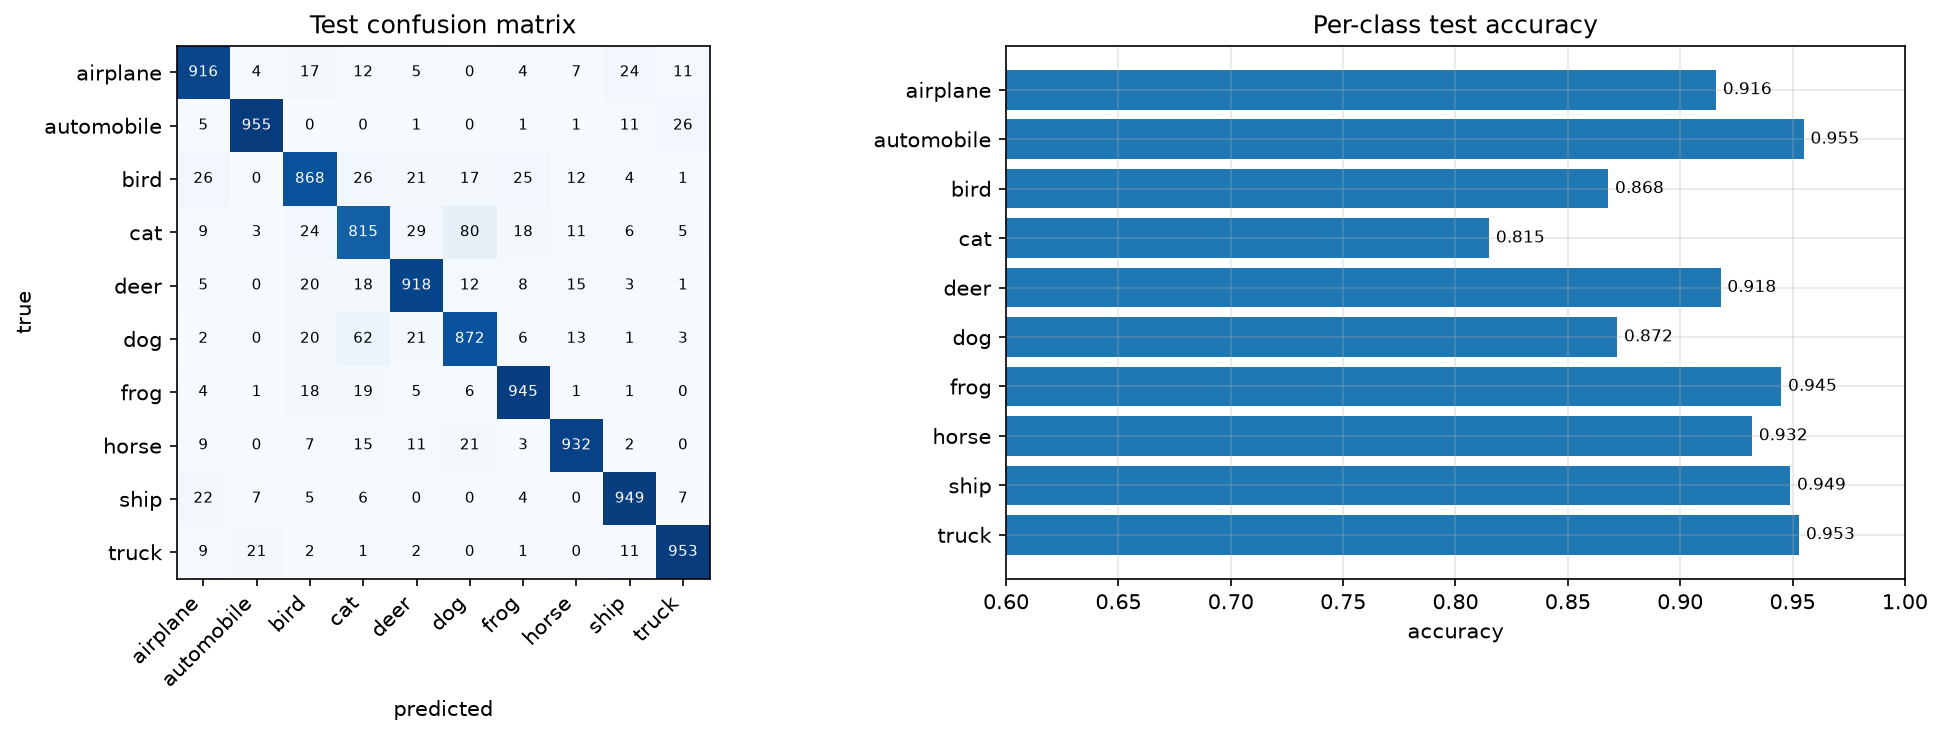
\includegraphics[width=\textwidth]{t4_test_confusion.png}
  \caption{Test-set confusion matrix and per-class accuracy of the final model.}
\end{figure}

\textbf{Interpretation.}
\begin{itemize}
  \item \textbf{Augmentation} is the most important choice ($-3.58$ points without it). Without it the training accuracy reaches 100\,\% by epoch 20, a clear overfit.
  \item \textbf{Weight decay} is second ($-1.68$). With batch norm, it keeps the weight norms small and so the effective learning rate high, which helps both optimization and generalization.
  \item \textbf{AdamW} is competitive but slightly below well-tuned SGD-Nesterov with one-cycle, a common result for CNNs on CIFAR.
  \item \textbf{Shortcuts} have only a small effect at 14 layers, consistent with 3(b), where they mattered little at depth 8--20 and a lot at depth 56.
  \item \textbf{Cutout and label smoothing hurt in this budget.}
  \begin{itemize}
    \item With cutout, training accuracy is only 87.9\,\%, against 95.3\,\% without it.
    \item Both are regularizers that pay off in long schedules. With 20 epochs the model is limited by under-training, not overfitting: the same bias--variance trade-off as 3(a)'s ``all combined''.
  \end{itemize}
  \item \textbf{Test vs.\ validation:} the test accuracy (91.23\,\%) is within half a point of the validation accuracy (90.78\,\%), which is within the sampling noise of a 5k validation set. Model selection did not overfit the validation split.
  \item \textbf{Errors:}
  \begin{itemize}
    \item Cat is the hardest class (81.5\,\%), mostly confused with dog (80 cats predicted as dogs, 62 dogs as cats).
    \item Other confusions are automobile $\leftrightarrow$ truck and airplane $\leftrightarrow$ ship.
    \item Vehicles are easiest: automobile 95.5\,\%, truck 95.3\,\%, ship 94.9\,\%.
  \end{itemize}
\end{itemize}

% ====================================================================
\section*{Conclusion}
\begin{itemize}
  \item \textbf{Backpropagation:} the from-scratch layers are verified to $10^{-17}$ (autograd) and $10^{-9}$ (finite differences). Sigmoid gradients vanish by about $10^5$ over 10 layers, while ReLU with He initialization keeps them balanced.
  \item \textbf{Optimizers:} the custom SGD-momentum and Adam match PyTorch exactly. Momentum and Adam fix ill-conditioning in different ways, and each optimizer works only within about one decade of learning rate.
  \item \textbf{Regularization:} with 5k images, geometric augmentation is the strongest regularizer, and stacking every regularizer underfits.
  \item \textbf{Residual connections:} plain-56 suffers from the degradation problem, while residual-56 is the best network. Shortcuts make depth usable.
  \item \textbf{Best CNN:} a 482k-parameter ResNet-14 trained for 20 epochs reaches \textbf{91.23\,\% test accuracy}. The ablation shows that augmentation and weight decay matter most.
\end{itemize}

\end{document}
